\documentclass[12pt, lettersize]{article}

\usepackage{graphicx} %to insert images
\graphicspath{ {}{} }%specify image location path. leave empty if images are on the same folder as the .tex source.
 
%usage: \begin{figure}
%\centering 
%\includegraphics[width= (*scale*) \linewidth]{imagefile}
%\end{figure}

\usepackage{amsfonts}
\usepackage{amssymb}
\usepackage{amsmath}
\usepackage{amsthm}
\usepackage{amsfonts}
\usepackage{amscd}
\usepackage{comment}
\usepackage{color}

\usepackage{enumerate}
%to use personalized enumerations 
%usage: \begin{enumerate}[*listing style you want. ex: i*]
%content...
%\end{enumerate}

\theoremstyle{Remark}
\newtheorem*{remark}{Remark}

\usepackage{pgfplots}


\usepackage[utf8]{inputenc}



\usepackage{listings}
\usepackage{xcolor}

\usepackage{geometry}

\definecolor{codegreen}{rgb}{0,0.6,0}
\definecolor{codegray}{rgb}{0.5,0.5,0.5}
\definecolor{codepurple}{rgb}{0.58,0,0.82}
\definecolor{backcolour}{rgb}{0.95,0.95,0.92}

\lstdefinestyle{mystyle}{
	backgroundcolor=\color{backcolour},   
	commentstyle=\color{codegreen},
	keywordstyle=\color{magenta},
	numberstyle=\tiny\color{codegray},
	stringstyle=\color{codepurple},
	basicstyle=\ttfamily\footnotesize,
	breakatwhitespace=false,         
	breaklines=true,                 
	captionpos=b,                    
	keepspaces=true,                 
	numbers=right,                    
	numbersep=5pt,                  
	showspaces=false,                
	showstringspaces=false,
	showtabs=false,                  
	tabsize=2
}

\lstset{style=mystyle} %to insert code directly from file.
%usage: \lstinputlisting[language = *language*, firstline = *first line to insert, lastline= *last line to insert]{filename}

\geometry{
	total={170mm,230mm},
	left=20mm,
	top=20mm,
}

\newcommand{\R}{\mathbb{R}}
\newcommand{\N}{\mathbb{N}}
\newcommand{\Z}{\mathbb{Z}}
\newcommand{\C}{\mathbb{C}}
\newcommand{\Q}{\mathbb{Q}}
\newcommand{\answertrue}{\color{red}\textbf{T}}
\newcommand{\answerfalse}{\color{red}\textbf{F}}

\setlength\parindent{0pt}


\title{\Large \centering{Database Project  } \\ \large \textbf{ CSI2132 Section A \\  Professor: Dr. Paula Branco} }

\author{ \large \textbf{Students:} Christopher Aris \\ 
	\texttt{300031710, caris015@uottawa.ca} \\
	Lev C. Guzman Aparicio \\
	\texttt{300038033, lguzm038@uottawa.ca}
	}


\begin{document}
	\begin{titlepage}
		\maketitle
	\end{titlepage}

	\section{Languages Used}
	
	To build the database project, the team used a combination of Python and SQL PostgreSQL flavour.
	In addition, to build the web application interface, the team used CLI in order to ensure correctness. \\
	
	The following DDLs were used in order to create our database:
	
	\begin{itemize}
		
		\item CREATE TABLE ... (...);
		
		\item ALTER TABLE (...);
		
		\item  ALTER COLUMN ... TYPE ...;
		
		\item RENAME ... TO ...;
		
		\item ADD CONSTRAINT ... FOREIGN KEY (...) REFERENCES ...(...) ON DELETE ... ON UPDATE ...;
		
		\item ADD COLUMN ...;
		
		\item ADD CONSTRAINT ... CHECK (...);
		
		\item ADD CONSTRAINT ... PRIMARY KEY (...);
		
		\item  ADD CONSTRAINT ... NOT NULL(...);
		
		\item DROP CONSTRAINT;
		
		\item DROP COLUMN;
		
	\end{itemize}

	\newpage

	\section{Queries}
	Ten queries were requested for our database. We present their code and the corresponding results
	
	\begin{enumerate}
		
		\item 
		\lstinputlisting[language= SQL, firstline = 3,lastline = 7]{QUERIES.sql}
		
		\begin{figure}[h]
			\centering
			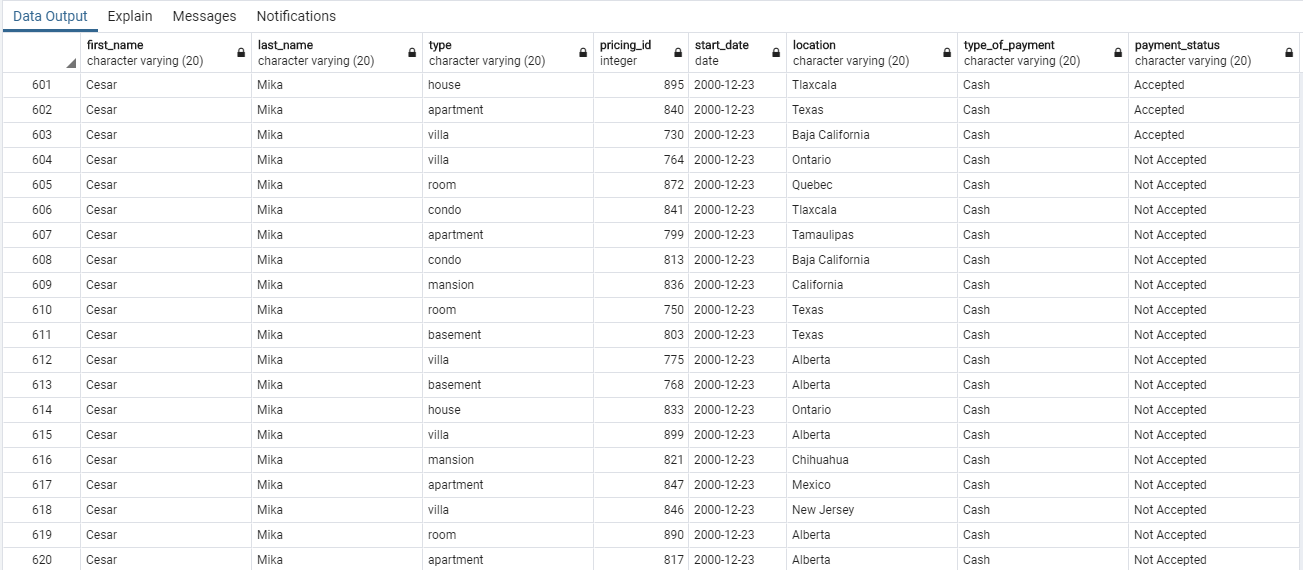
\includegraphics[width= \linewidth]{Query1Output.png}
			\caption{Output of the 1st Query}
		\end{figure}
		
		\newpage
		
		\item 
		\lstinputlisting[language= SQL, firstline = 9,lastline = 13]{QUERIES.sql}
		
		\begin{figure}[h]
		\centering
		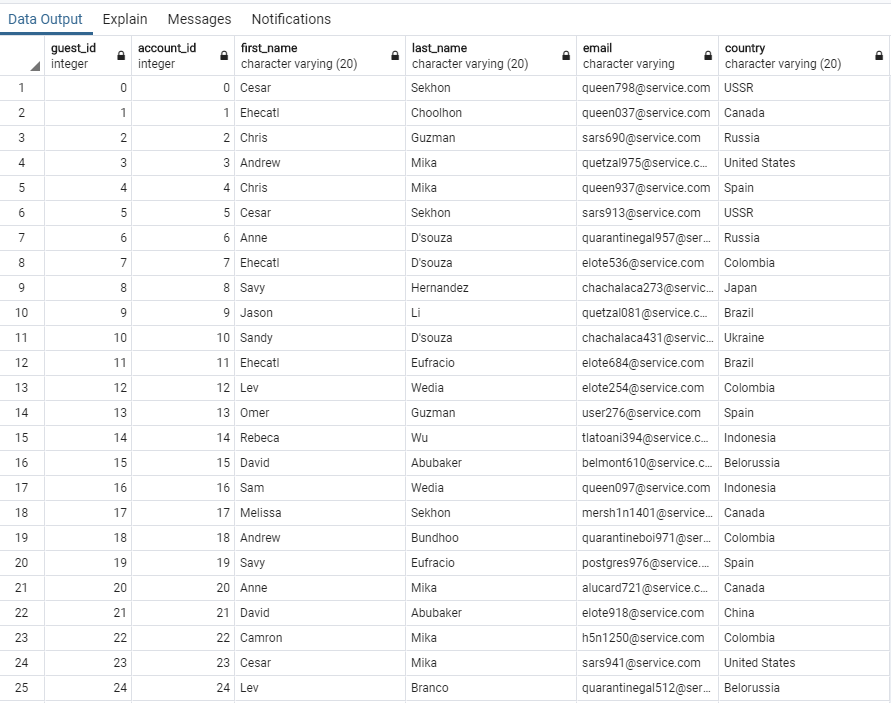
\includegraphics[width= \linewidth]{Query2Output.png}
		\caption{Output of the 2nd Query}
		\end{figure}

		\item 
		\lstinputlisting[language= SQL, firstline = 15,lastline = 18]{QUERIES.sql}
		
		\begin{figure}[h]
			\centering
			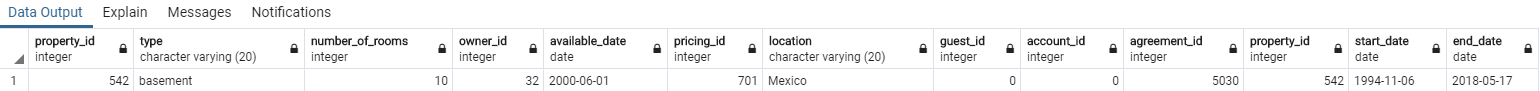
\includegraphics[width= \linewidth]{Query3Output.png}
			\caption{Output of the 3nd Query}
		\end{figure}
	
		
		\item 
		\lstinputlisting[language= SQL, firstline = 20,lastline = 25]{QUERIES.sql}
		
		\begin{figure}[h]
			\centering
			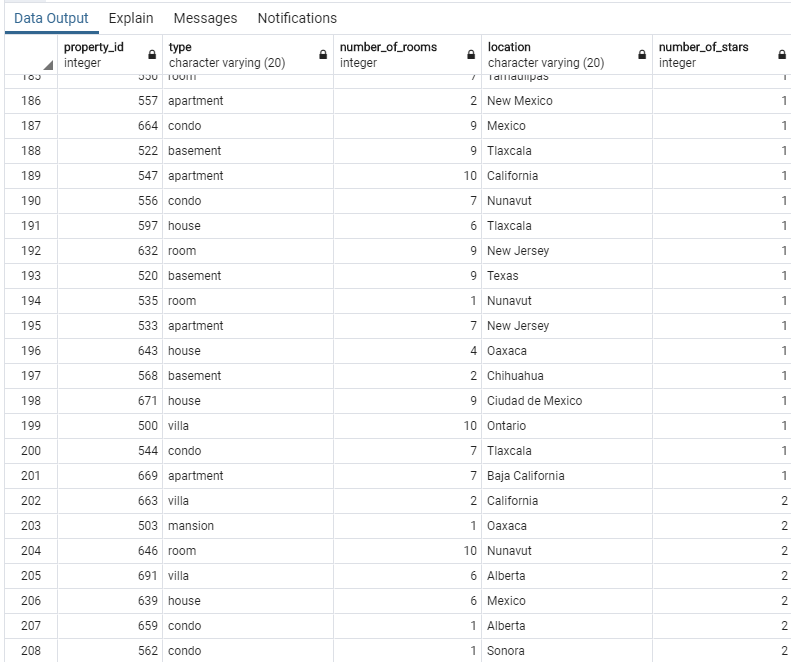
\includegraphics[width= 0.8\linewidth]{Query4Output.png}
			\caption{Output of the 4th Query.}
		\end{figure}
				
		\newpage
		
		\item 
		\lstinputlisting[language = SQL, firstline = 1, lastline = 4 ]{Query5.sql}
		
		\begin{figure}[h]
			\centering
			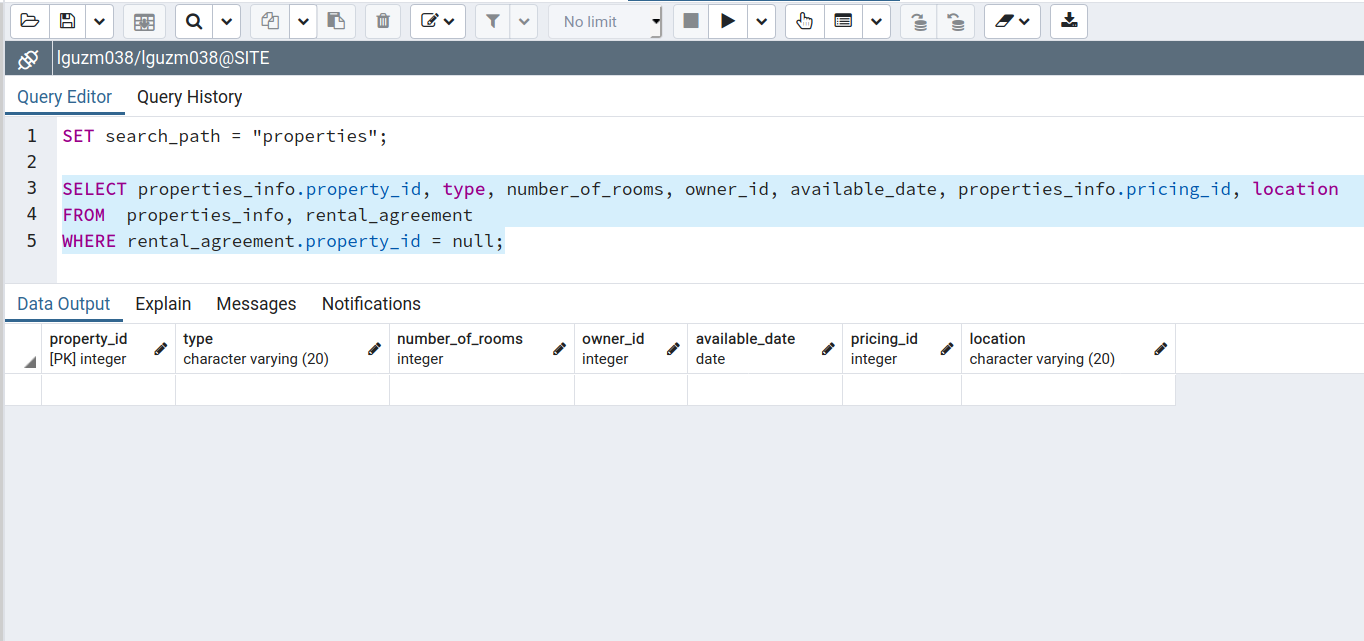
\includegraphics[width= 0.8\linewidth]{Query5Output.png}
			\caption{Output of the 5th Query. Note that it is empty since we inserted no null values}
		\end{figure}
		
		
		
		\item 
		\lstinputlisting[language= SQL, firstline = 27,lastline = 30]{QUERIES.sql}
		
		\begin{figure}[h]
			\centering
			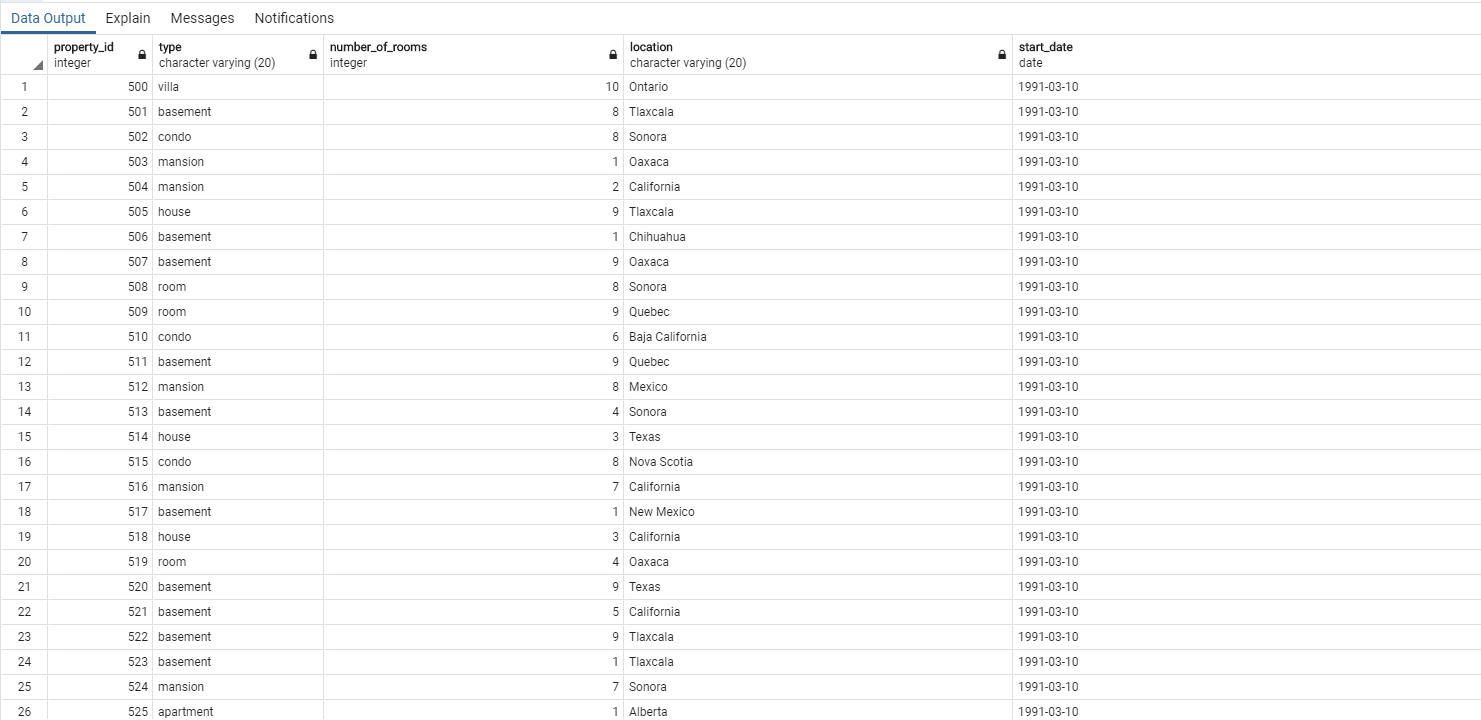
\includegraphics[width= 0.8\linewidth]{Query6Output.png}
			\caption{Output of the 6th Query.}
		\end{figure}
	
		\newpage
		
		\item 
		\lstinputlisting[language= SQL, firstline = 32,lastline = 36]{QUERIES.sql}
		
		\begin{figure}[h]
			\centering
			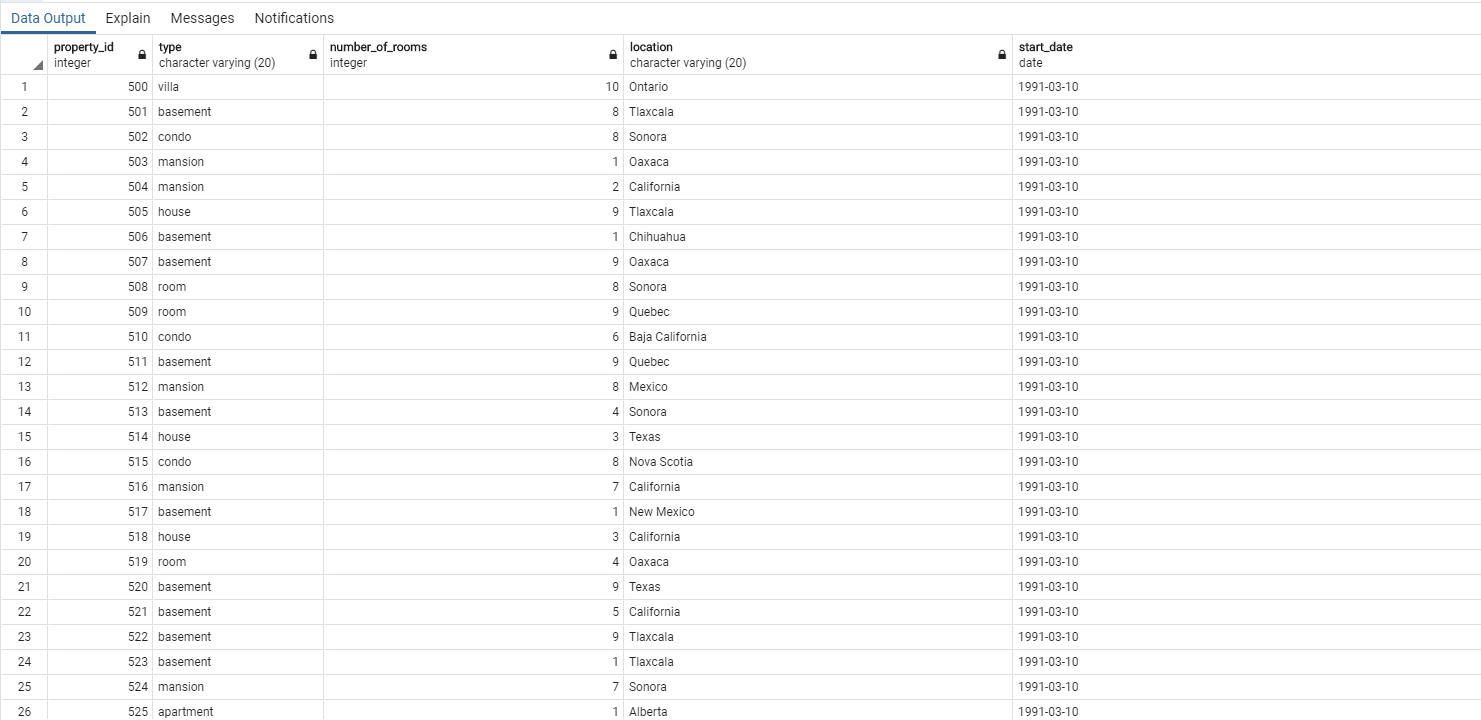
\includegraphics[width= 0.8\linewidth]{Query6Output.png}
			\caption{Output of the 7th Query.}
		\end{figure}
		
		\newpage
		
		\item 
		\lstinputlisting[language= SQL, firstline = 38,lastline = 41]{QUERIES.sql}
		
		\begin{figure}[h]
			\centering
			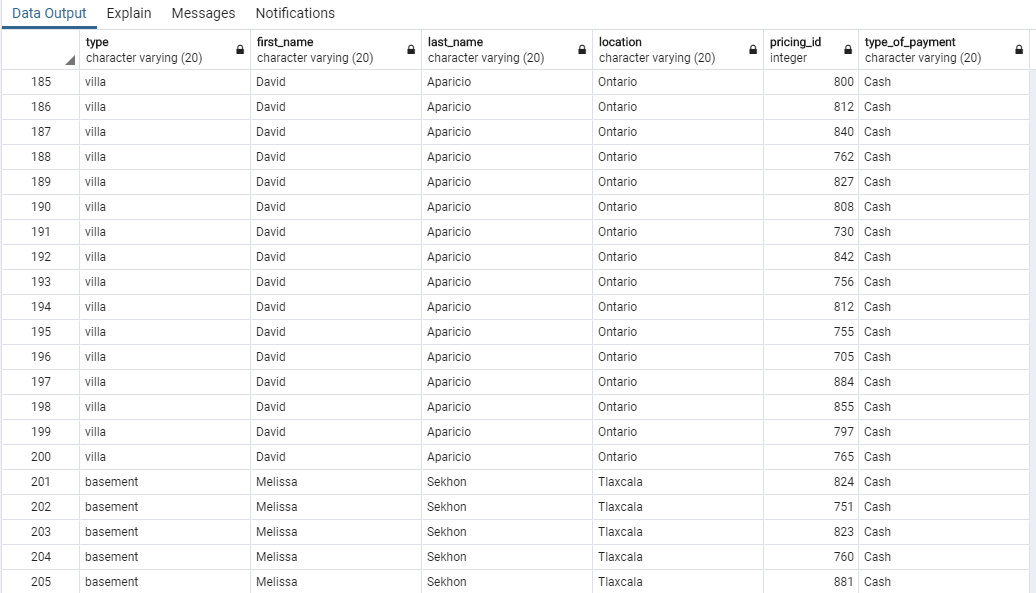
\includegraphics[width= 0.7\linewidth]{Query8Output.png}
			\caption{Output of the 8th Query.}
		\end{figure}
		
		\item 
		\lstinputlisting[language= SQL, firstline = 43,lastline = 47]{QUERIES.sql}
		
		\begin{figure}[h]
			\centering
			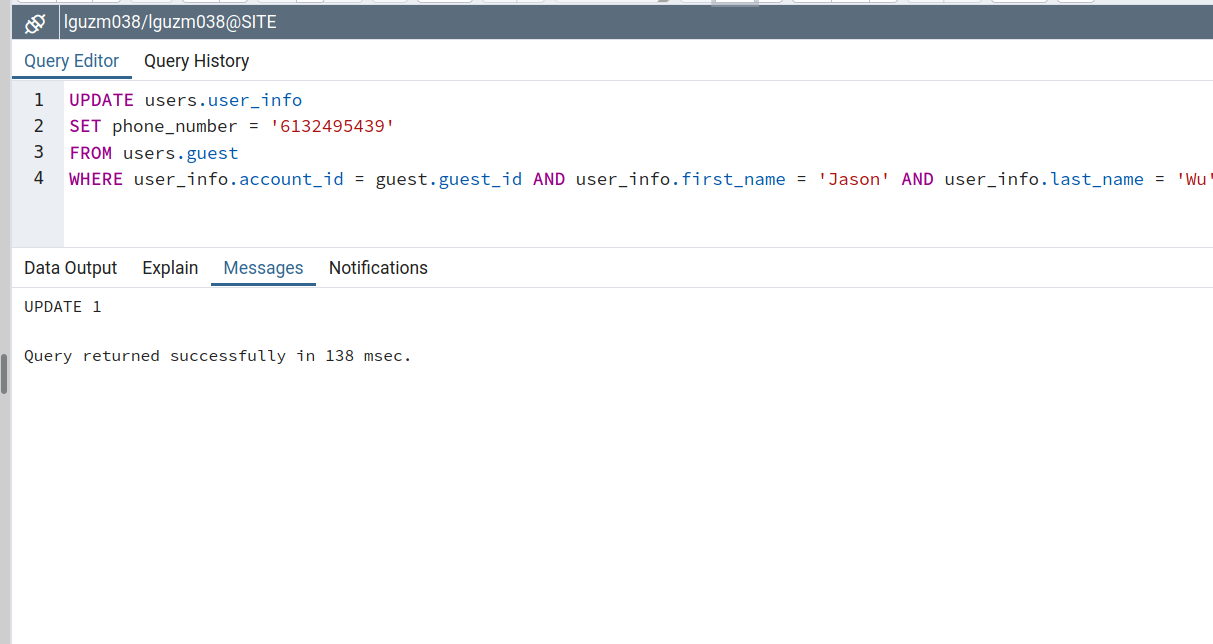
\includegraphics[width= 0.6\linewidth]{Query9Output.png}
			\caption{Output of the 9th Query.}
		\end{figure}
		
		\item 
		\lstinputlisting[language= SQL, firstline = 48,lastline = 53]{QUERIES.sql}
		
		\begin{figure}[h]
			\centering
			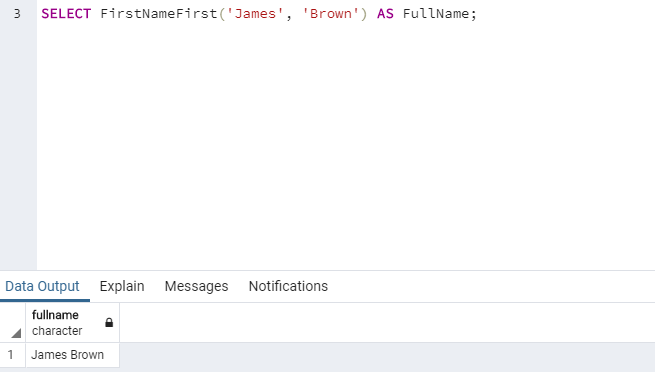
\includegraphics[width= 0.6\linewidth]{Query10Output.png}
			\caption{Output of the 10th Query.}
		\end{figure}
		
	\end{enumerate}
	

	
		
	\section{How to Install}
	
	To set up the database we must follow these steps in order:
	
	\begin{itemize}
		\item Restore the provided backup file in order to access the schema and tables.
		
		\item In the \textsl{Data} folder, execute the provided python script \textbf{data\_insertor.py} with the following command: \texttt{python3 data\_insertor.py} 
		
		\item Now de database is populated.
		
	\end{itemize}	
	
		 
	 To install the CLI tool it is \textbf{important} that the guide is followed strictly in order to make sure that no errors present themselves.
	 
	 \begin{itemize}
	 	
	 	\item It is \textsl{strongly} advised that the program is ran in a virtual environment
	 	
	 	\item It is \textbf{even more so} advised that this installation is executed using the latest version of Python, but any Python 3.X version will suffice.
	 	
	 	\begin{remark}
	 		Please \textbf{do not use} Python 2.X binaries because there \textbf{WILL} be errors.
	 	\end{remark}
	 	
	 	\item  Once in a virtual environment run the command: \texttt{pip install --editable}. \\
	 	What this is essentially telling Python is to install the package in the current directory (which you guessed it, is our CLI Tool), the editable option will link the package to the directory location and mitigate any nasty import errors.
	 	
	 	\item If on a UNIX system you might have to run the following instead:
	 	\texttt{pip3 install --editable}. 
	 	This specifies to your system to select a Python 3.X version if a Python 2.X is also installed (which is usally the case with Linux distros)
	 	
	 	\item Once installed verify installation by checking for the package `travelCLI   v1.0`
	 	To do this, type \texttt{pip list} or \texttt{pip3 list} (if on a UNIX system)
	 	
	 	\item To finally start using the CLI Tool, the binding keyword is \texttt{controller} so if I were to run the check command I would do like so:
	 	\texttt{\$ controller check}
	 	
	 	\begin{remark}
	 		Note that you will need to edit the configuration file titled `database.ini` to change the credentials to appropriate ones; in order to connect to the proper database source.
	 	\end{remark}
	 	
	 \end{itemize}
	 
 
	
\end{document}
